%\documentclass[10pt]{article}
\documentclass[fleqn]{article}
%\usepackage[cm]{fullpage}
\usepackage{graphicx}
\usepackage{amsmath}
\usepackage{outlines}
\usepackage{listings}
\usepackage{xcolor}
\lstset { %
	language=R,
	backgroundcolor=\color{black!5}, % set backgroundcolor
	basicstyle=\footnotesize,% basic font setting
}

%Regression table preamp

\usepackage{booktabs} % For \toprule, \midrule and \bottomrule
\usepackage{siunitx} % Formats the units and values
\usepackage{pgfplotstable} % Generates table from .csv
\usepackage{booktabs}

% Setup siunitx:
\sisetup{
	round-mode          = places, % Rounds numbers
	round-precision     = 4, % to 2 places
}

\usepackage{float}

\title{Housing and Credit Cycles}
\author{Nam Nguyen}
\date{\today}                                          

\begin{document}
	\maketitle
	
\begin{outline}[enumerate]

\section{Motivation}

This paper uses a multivariate extension of the model proposed by Morley et al. (2003) and Huang and Kishor (2018)

The novel contribution of this paper is the inclusion of cross transitory components effect as seen in eq(5) \& eq(6). I would like to take advantage of it to explore the dynamics of the relationship between housing prices and house hold credit in the short run.
		
\section {Model Specification}

\textbf{\textit{Series:}} \\
-Credit : Credit to non financial sector\\
-HPI : Housing Price Index
	\begin{align}
	ln \frac{Credit}{GDP} &= y_t = \tau_{yt} + c_{yt}
	\\
	ln HPI &= h_t = \tau_{ht} + c_{ht}
	\end{align}
	\\
\textbf{\textit{Trends:}}

A random walk drift term $g_t$ is added in the stochastic trend inspired by Clark (1987)
	\begin{align}
	\tau_{yt} &= \tau_{yt-1} + \eta_{yt}, &\eta_{yt} \sim iidN(0,\sigma^2_{\eta y})
	\\
	\tau_{ht} &= \tau_{ht-1} + \eta_{ht}, &\eta_{ht} \sim iidN(0,\sigma^2_{\eta h})	
	\end{align}
	\\
\textbf{\textit{Cycles:}}
	\begin{align}
	c_{yt} &= \phi^1_{y}c_{yt-1}  
		   + \phi^2_{y}c_{yt-2}  
		   + \phi^x_{y}c_{ht-1} 
		   + \varepsilon_{yt},
		   &\varepsilon_{yt} \sim iidN(0,\sigma^2_{\varepsilon y})		   
	\\
	c_{ht} &= \phi^1_{h}c_{ht-1}  
		   + \phi^2_{h}c_{ht-2}
		   + \phi^x_{h}c_{yt-1}  
	   	   + \varepsilon_{ht},
	   	   	&\varepsilon_{ht} \sim iidN(0,\sigma^2_{\varepsilon h})
	\end{align}
	\\


\textbf{State-Space Model}

\textit{Transition equation:}
\begin{align}
\beta_t = F\beta_{t-1} + \tilde{v}_t
\end{align}

Where the transitory components are:

\begin{align}
\begin{bmatrix}
\tau_{yt}	\\
c_{yt}		\\
c_{yt-1}		\\
\tau_{ht}	\\
c_{ht}		\\
c_{ht-1}		
\end{bmatrix}
=
%F matrix
\begin{bmatrix}
1	& 0	& 0	& 0	& 0	& 0	\\
0	& \phi^1_y	& \phi^2_y	& 0	& \phi^x_y	& 0	\\
0	& 1	& 0	& 0 & 0 & 0  \\
0	& 0	& 0	& 1	& 0	& 0 \\
0	& \phi^x_h	& 0	& 0 &\phi^1_h	& \phi^2_h	\\
0	& 0	& 0	& 0 & 1 & 0
\end{bmatrix}
%Bt-1 matrix
\begin{bmatrix}
\tau_{yt-1}	\\
c_{yt-1}		\\
c_{yt-2}		\\
\tau_{ht-1}	\\
c_{ht-1}		\\
c_{ht-2}		
\end{bmatrix}
+
\begin{bmatrix}
\eta_{yt}	\\
\varepsilon_{yt}		\\
0	\\
\eta_{ht}	\\
\varepsilon_{ht}		\\
0	
\end{bmatrix}
\end{align}

\textit{The covariance matrix for $\tilde{v}_t$, denoted Q, is: }
\begin{align}
Q = 
\begin{bmatrix}
\sigma^2_{\eta y}	& 0	 &0 & 0	& 0	& 0	\\
0	& \sigma^2_{\varepsilon y}	& 0	& 0	& \sigma_{\varepsilon y \varepsilon h}	& 0	\\
0	&	0	& 0 & 0 & 0 & 0	\\
0	& 0	& 0	& \sigma^2_{\eta h}	& 0	& 0	\\
0	& \sigma_{\varepsilon y \varepsilon h}	& 0	& 0	& \sigma^2_{\varepsilon h}		& 0	\\
0	&0	& 0	& 0
	& 0	& 0
\end{bmatrix}
\end{align}

\textit{Measurement Equation:}
\begin{align}
\tilde{y}_t = A + H\beta_t
\end{align}

\begin{align*}
\begin{bmatrix}
y_t	\\
h_t
\end{bmatrix}
=
\begin{bmatrix}
0	\\
0
\end{bmatrix}
+
\begin{bmatrix}
1	& 0	& 1	& 0	& 0 & 0 \\
0	& 0 & 0 & 1 & 0 & 1
\end{bmatrix}
\begin{bmatrix}
\tau_{yt}	\\
c_{yt}		\\
c_{yt-1}	\\
\tau_{ht}	\\
c_{ht}		\\
c_{ht-1}
\end{bmatrix}
\end{align*}
\pagebreak
\section{Parameters constraints}

The estimation of the unobserved component model uses a nonlinear log-likelihood function maximization. Estimating this function requires numerical optimization.


Following Kim \& Nelson Chap 2, I set up the constraints on the autoregressive parameters to imply stationary and $-1<\phi^{y}_{x}<1$ as follow:

\begin{align*}
\phi^{y}_{x} &= \frac{\phi^{y}_{x}}{1+|{\phi^{y}_{x}|}} &\phi^{h}_{x} = \frac{\phi^{h}_{x}}{1+|{\phi^{h}_{x}|}}
\end{align*}

\vspace{5mm} %5mm vertical space

Regarding constraints on covariance matrix, I applied the same constraints as in Morley 2007 to imply for positive definite matrix, in order to ensure feasible maximum likelihood estimation process. Furthermore, I suppressed the cross trend covariance term to be zero.



\section{Regression results}

In this following section, I will apply the UC model to data from 6 countries: US, UK, Germany, France, Japan and South Korea.

The estimated parameters vary greatly as I uniformly randomized priors for the MLE process. The following estimates are selected in the manner that they would look the most stable. Perhaps a more optimal constraint on the autoregressive parameters would solve this issue.

\pagebreak

\pgfplotstableset{% global config, for example in the preamble
	every last row/.style={after row=\bottomrule}
}

%Regression table
\begin{table*}
	\begin{center}
	\caption{Correlated UC model Estimates: US data}
	\begin{tabular}{c}
		\toprule
		Description\\
		\midrule
		$\phi^1_{y}$ \\
%		$\phi^2_{y}$ \\		
%		$\phi^x_{y}$ \\
		$\phi^1_{h}$ \\
%		$\phi^2_{h}$ \\		
%		$\phi^x_{h}$ \\
		$\sigma_{ny}$\\
		$\sigma_{ey}$\\
		$\sigma_{nh}$\\
		$\sigma_{eh}$\\
		$\sigma_{eyeh}$\\
		$\sigma_{nynh}$\\
%		$\mu$\\
		Log-likelihood value\\
		\bottomrule
	\end{tabular}%
        \pgfplotstabletypeset[
        multicolumn names, % allows to have multicolumn names
        col sep= comma, % the seperator in our .csv file
        display columns/0/.style={
        	column name=Estimate, % name of first column
        	column type={S},string type},  % use siunitx for formatting
        display columns/1/.style={
        	column name=Standard Error,
        	column type={S},string type},
        every head row/.style={
        	before row={\toprule}, % have a rule at top
        	after row={
        		%\si{\ampere} & \si{\volt}\\ % %the units seperated by &
        		\midrule} % rule under units
        },
        every last row/.style={after row=\bottomrule}, % rule at bottom
        ]{../Output/Reg_US.csv} % filename/path to file
	\end{center}
\end{table*}

\begin{table*}
	\begin{center}
		\caption{Correlated UC model Estimates: UK data}
		\begin{tabular}{c}
		\toprule
		Description\\
		\midrule
		$\phi^1_{y}$ \\
		$\phi^2_{y}$ \\		
%		$\phi^x_{y}$ \\
		$\phi^1_{h}$ \\
		$\phi^2_{h}$ \\		
%		$\phi^x_{h}$ \\
		$\sigma^2_{ny}$\\
		$\sigma^2_{ey}$\\
		$\sigma^2_{nh}$\\
		$\sigma^2_{eh}$\\
		$\sigma_{eyeh}$\\
		$\sigma_{nynh}$\\
%		$\mu$\\
		Log-likelihood value\\
		\bottomrule
		\end{tabular}%
		\pgfplotstabletypeset[
		multicolumn names, % allows to have multicolumn names
		col sep= comma, % the seperator in our .csv file
		display columns/0/.style={
			column name=Estimate, % name of first column
			column type={S},string type},  % use siunitx for formatting
		display columns/1/.style={
			column name=Standard Error,
			column type={S},string type},
		every head row/.style={
			before row={\toprule}, % have a rule at top
			after row={
				%\si{\ampere} & \si{\volt}\\ % %the units seperated by &
				\midrule} % rule under units
		},
		every last row/.style={after row=\bottomrule}, % rule at bottom
		]{../Output/Reg_GB.csv} % filename/path to file
	\end{center}
\end{table*}
%
%\begin{table*}
%	\begin{center}
%		\caption{Correlated UC model Estimates: Germany data}
%		\begin{tabular}{c}
%			\toprule
%			Description\\
%			\midrule
%			$\phi^y_{1}$ \\
%			$\phi^y_{x}$ \\		
%			$\phi^h_{1}$ \\
%			$\phi^h_{x}$ \\
%			$\sigma^2_{ny}$\\
%			$\sigma^2_{wy}$\\
%			$\sigma^2_{ey}$\\
%			$\sigma^2_{nh}$\\
%			$\sigma^2_{wh}$\\
%			$\sigma^2_{eh}$\\
%			$\sigma_{nhnc}$\\
%			$\sigma_{ehec}$\\
%			Log-likelihood value\\
%			\bottomrule
%		\end{tabular}%
%		\pgfplotstabletypeset[
%		multicolumn names, % allows to have multicolumn names
%		col sep= space, % the seperator in our .csv file
%		display columns/0/.style={
%			column name=Estimate, % name of first column
%			column type={S},string type},  % use siunitx for formatting
%		display columns/1/.style={
%			column name=Standard Error,
%			column type={S},string type},
%		every head row/.style={
%			before row={\toprule}, % have a rule at top
%			after row={
%				%\si{\ampere} & \si{\volt}\\ % %the units seperated by &
%				\midrule} % rule under units
%		},
%		every last row/.style={after row=\bottomrule}, % rule at bottom
%		]{../Output/Reg_DE.csv} % filename/path to file
%	\end{center}
%\end{table*}
%
%\begin{table*}
%	\begin{center}
%		\caption{Correlated UC model Estimates: France data}
%		\begin{tabular}{c}
%			\toprule
%			Description\\
%			\midrule
%			$\phi^y_{1}$ \\
%			$\phi^y_{x}$ \\		
%			$\phi^h_{1}$ \\
%			$\phi^h_{x}$ \\
%			$\sigma^2_{ny}$\\
%			$\sigma^2_{wy}$\\
%			$\sigma^2_{ey}$\\
%			$\sigma^2_{nh}$\\
%			$\sigma^2_{wh}$\\
%			$\sigma^2_{eh}$\\
%			$\sigma_{nhnc}$\\
%			$\sigma_{ehec}$\\
%			Log-likelihood value\\
%			\bottomrule
%		\end{tabular}%
%		\pgfplotstabletypeset[
%		multicolumn names, % allows to have multicolumn names
%		col sep= space, % the seperator in our .csv file
%		display columns/0/.style={
%			column name=Estimate, % name of first column
%			column type={S},string type},  % use siunitx for formatting
%		display columns/1/.style={
%			column name=Standard Error,
%			column type={S},string type},
%		every head row/.style={
%			before row={\toprule}, % have a rule at top
%			after row={
%				%\si{\ampere} & \si{\volt}\\ % %the units seperated by &
%				\midrule} % rule under units
%		},
%		every last row/.style={after row=\bottomrule}, % rule at bottom
%		]{../Output/Reg_FR.csv} % filename/path to file
%	\end{center}
%\end{table*}
%
%\begin{table*}
%	\begin{center}
%		\caption{Correlated UC model Estimates: Japan data}
%		\begin{tabular}{c}
%			\toprule
%			Description\\
%			\midrule
%			$\phi^y_{1}$ \\
%			$\phi^y_{x}$ \\		
%			$\phi^h_{1}$ \\
%			$\phi^h_{x}$ \\
%			$\sigma^2_{ny}$\\
%			$\sigma^2_{wy}$\\
%			$\sigma^2_{ey}$\\
%			$\sigma^2_{nh}$\\
%			$\sigma^2_{wh}$\\
%			$\sigma^2_{eh}$\\
%			$\sigma_{nhnc}$\\
%			$\sigma_{ehec}$\\
%			Log-likelihood value\\
%			\bottomrule
%		\end{tabular}%
%		\pgfplotstabletypeset[
%		multicolumn names, % allows to have multicolumn names
%		col sep= space, % the seperator in our .csv file
%		display columns/0/.style={
%			column name=Estimate, % name of first column
%			column type={S},string type},  % use siunitx for formatting
%		display columns/1/.style={
%			column name=Standard Error,
%			column type={S},string type},
%		every head row/.style={
%			before row={\toprule}, % have a rule at top
%			after row={
%				%\si{\ampere} & \si{\volt}\\ % %the units seperated by &
%				\midrule} % rule under units
%		},
%		every last row/.style={after row=\bottomrule}, % rule at bottom
%		]{../Output/Reg_JP.csv} % filename/path to file
%	\end{center}
%\end{table*}
%
%\begin{table*}
%	\begin{center}
%		\caption{Correlated UC model Estimates: Korea data}
%		\begin{tabular}{c}
%			\toprule
%			Description\\
%			\midrule
%			$\phi^y_{1}$ \\
%			$\phi^y_{x}$ \\		
%			$\phi^h_{1}$ \\
%			$\phi^h_{x}$ \\
%			$\sigma^2_{ny}$\\
%			$\sigma^2_{wy}$\\
%			$\sigma^2_{ey}$\\
%			$\sigma^2_{nh}$\\
%			$\sigma^2_{wh}$\\
%			$\sigma^2_{eh}$\\
%			$\sigma_{nhnc}$\\
%			$\sigma_{ehec}$\\
%			Log-likelihood value\\
%			\bottomrule
%		\end{tabular}%
%		\pgfplotstabletypeset[
%		multicolumn names, % allows to have multicolumn names
%		col sep= space, % the seperator in our .csv file
%		display columns/0/.style={
%			column name=Estimate, % name of first column
%			column type={S},string type},  % use siunitx for formatting
%		display columns/1/.style={
%			column name=Standard Error,
%			column type={S},string type},
%		every head row/.style={
%			before row={\toprule}, % have a rule at top
%			after row={
%				%\si{\ampere} & \si{\volt}\\ % %the units seperated by &
%				\midrule} % rule under units
%		},
%		every last row/.style={after row=\bottomrule}, % rule at bottom
%		]{../Output/Reg_KR.csv} % filename/path to file
%	\end{center}
%\end{table*}

\clearpage
\section{Conclusion}
Employing cross effects on the transitory components of the two series allows me to measure the effect of short term shock from house hold credit on housing price and vice versa.  

For example, the model for US data shows that there is a positive relationship between a one period lag in short term house price and house hold credit. Also for the UK data, there is a positive relationship between a one period lag in short term credit and house price.

Further development for this paper should include more optimal constraints on parameters to ensure stability. 

Additionally, comparison in term of fitness and prediction error with other model such as a conventional multivariate UC model, univariate UC model, AR(2) model could be done in order gauge the benefit of including extra variables in the transitory component.

\begin{figure}[h!]
\caption{Appendix: US Credit components}	
\centerline{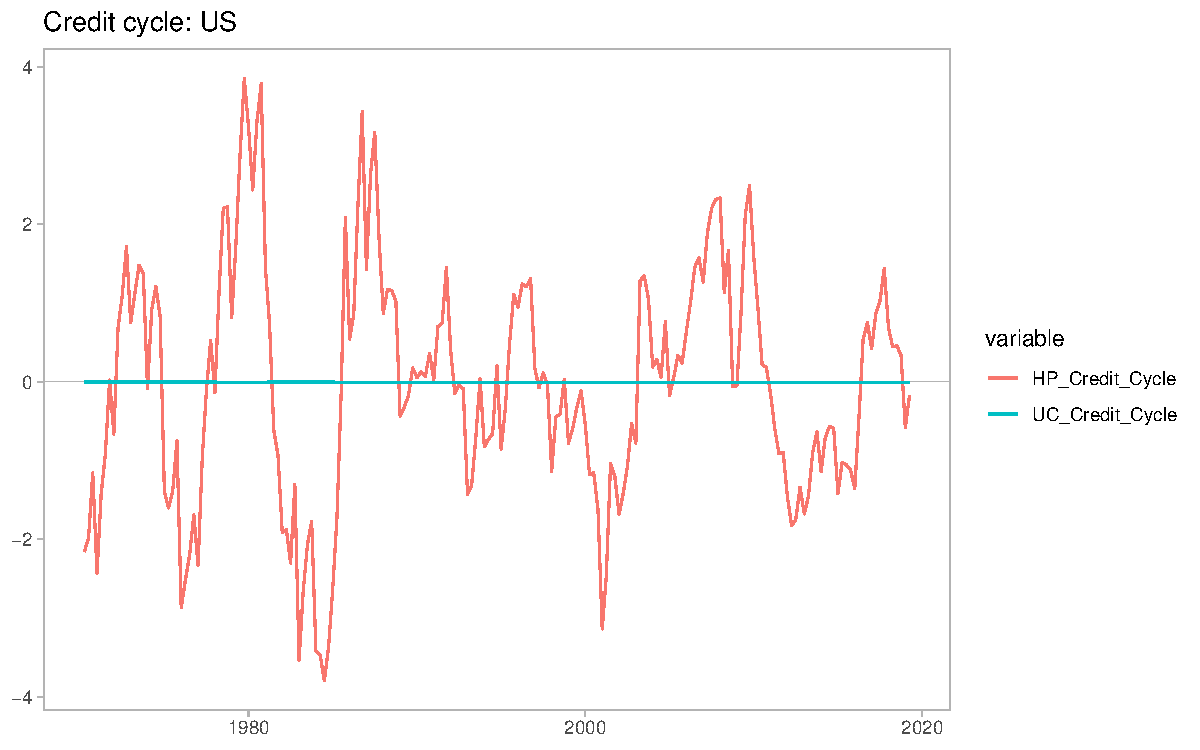
\includegraphics[scale=0.7]{../Output/Graphs/Credit_cycle_US.pdf}}
\centerline{\includegraphics[scale=0.7]{../Output/Graphs/Credit_trend_US.pdf}}
\end{figure}

\begin{figure}[h!]
\caption{US Housing Price components}	
\centerline{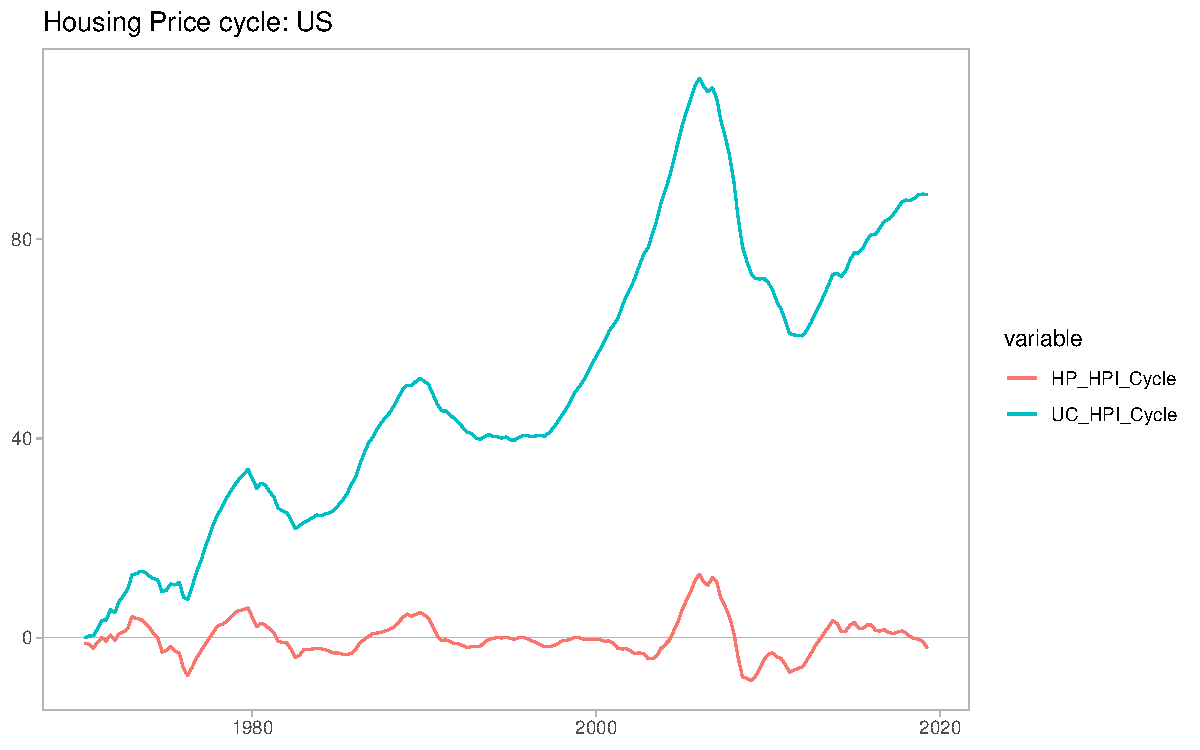
\includegraphics[scale=0.7]{../Output/Graphs/HP_cycle_US.pdf}}
\centerline{\includegraphics[scale=0.7]{../Output/Graphs/HP_trend_US.pdf}}
\end{figure}

\begin{figure}[h!]
	\caption{UK Credit components}	
	\centerline{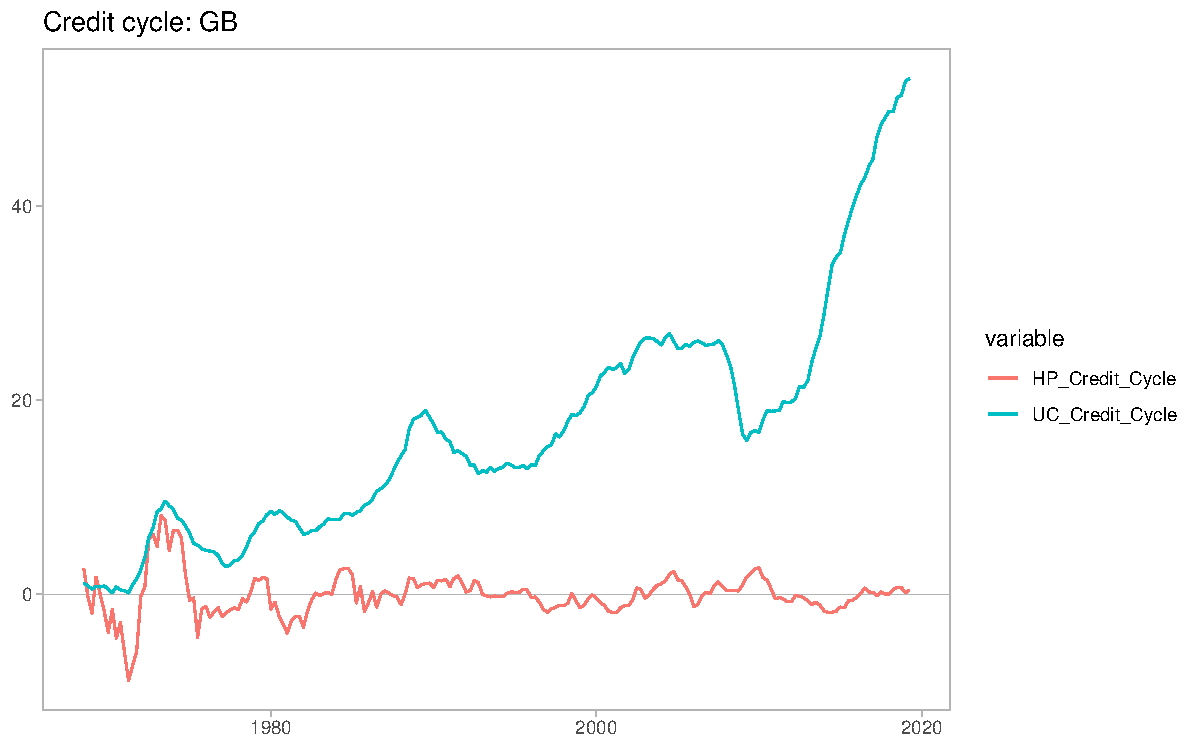
\includegraphics[scale=0.7]{../Output/Graphs/Credit_cycle_GB.pdf}}
	\centerline{\includegraphics[scale=0.7]{../Output/Graphs/Credit_trend_GB.pdf}}
\end{figure}

\begin{figure}[h!]
	\caption{UK Housing Price components}	
	\centerline{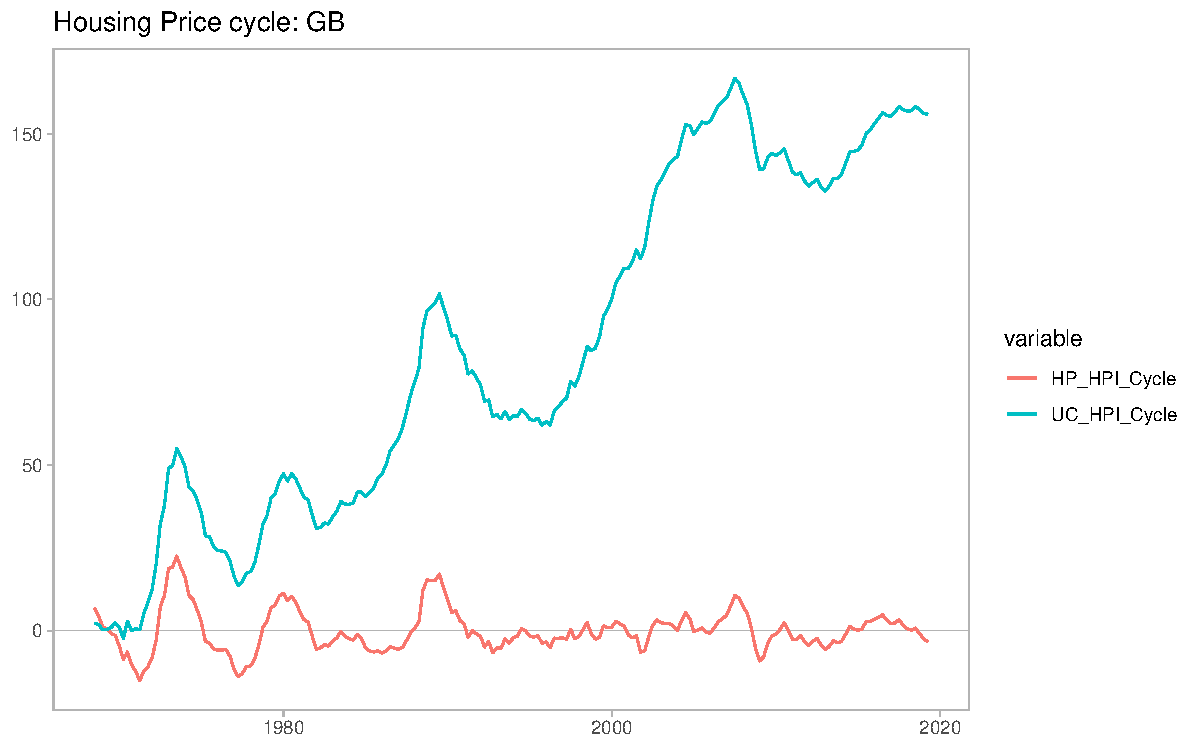
\includegraphics[scale=0.7]{../Output/Graphs/HP_cycle_GB.pdf}}
	\centerline{\includegraphics[scale=0.7]{../Output/Graphs/HP_trend_GB.pdf}}
\end{figure}

%
%\begin{figure}[h!]
%	\caption{Germany Credit components}	
%	\centerline{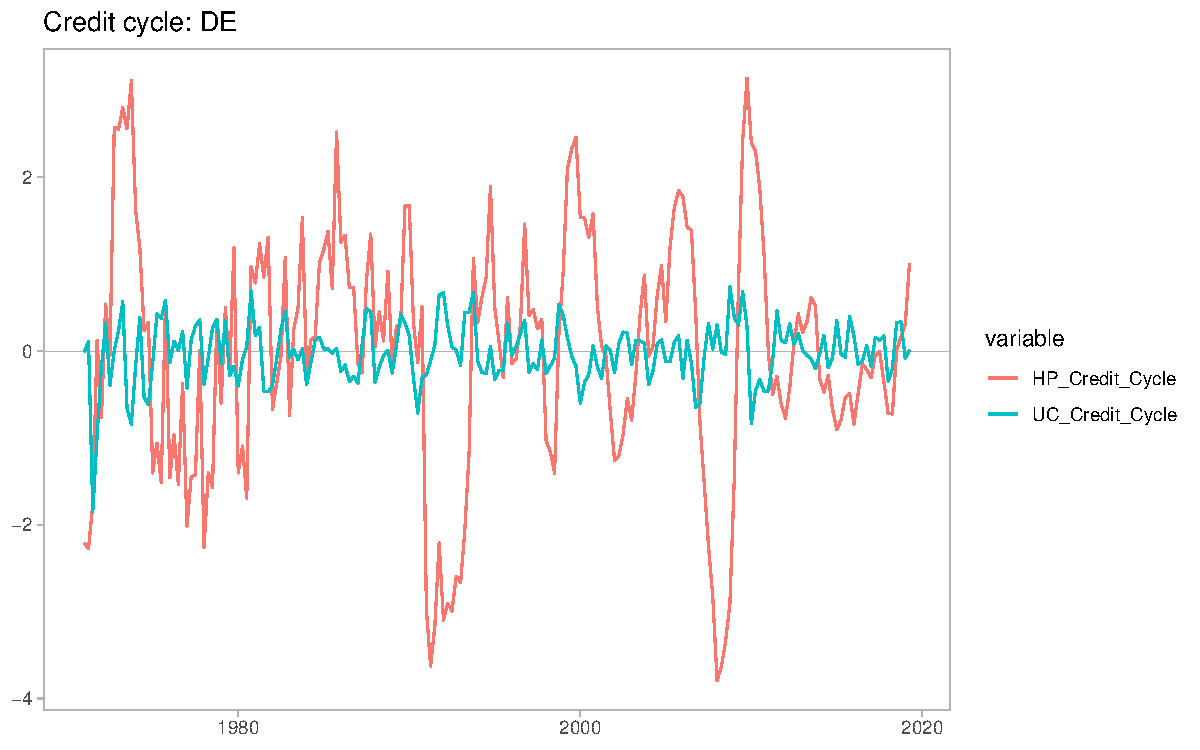
\includegraphics[scale=0.7]{../Output/Graphs/Credit_cycle_DE.pdf}}
%	\centerline{\includegraphics[scale=0.7]{../Output/Graphs/Credit_trend_DE.pdf}}
%\end{figure}
%
%\begin{figure}[h!]
%	\caption{Germany Housing Price components}	
%	\centerline{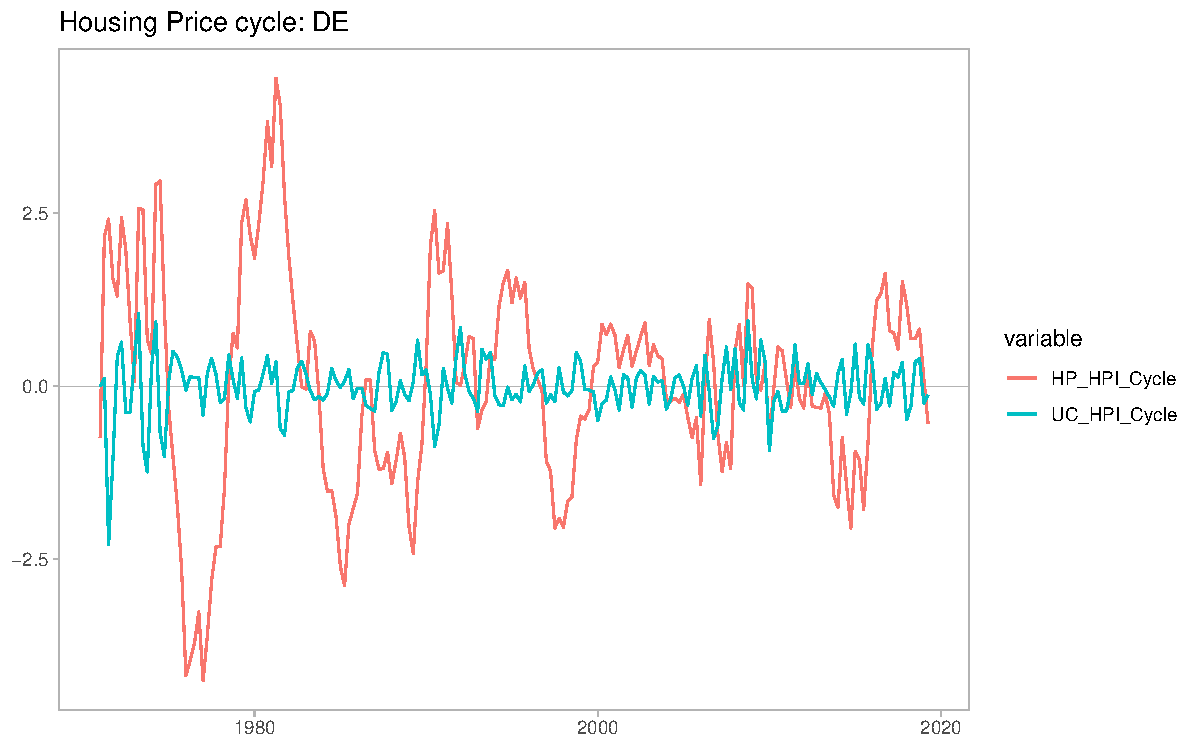
\includegraphics[scale=0.7]{../Output/Graphs/HP_cycle_DE.pdf}}
%	\centerline{\includegraphics[scale=0.7]{../Output/Graphs/HP_trend_DE.pdf}}
%\end{figure}
%
%
%\begin{figure}[h!]
%	\caption{France Credit components}	
%	\centerline{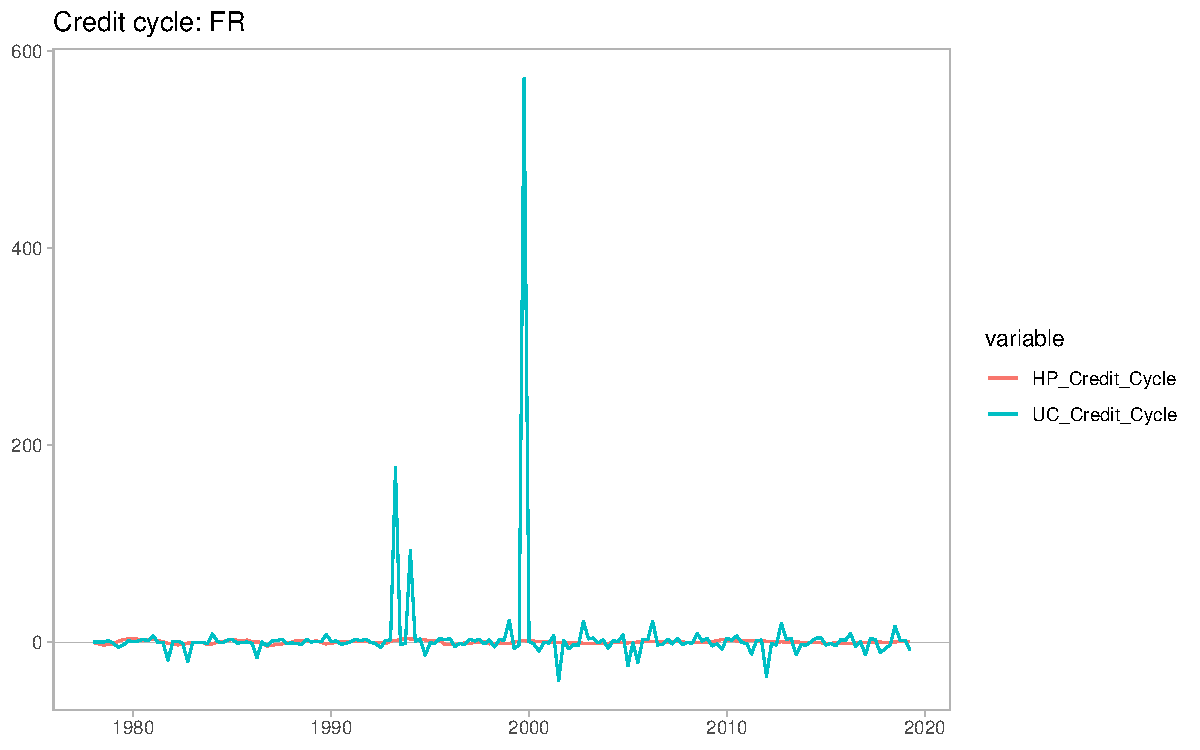
\includegraphics[scale=0.7]{../Output/Graphs/Credit_cycle_FR.pdf}}
%	\centerline{\includegraphics[scale=0.7]{../Output/Graphs/Credit_trend_FR.pdf}}
%\end{figure}
%
%\begin{figure}[h!]
%	\caption{France Housing Price components}	
%	\centerline{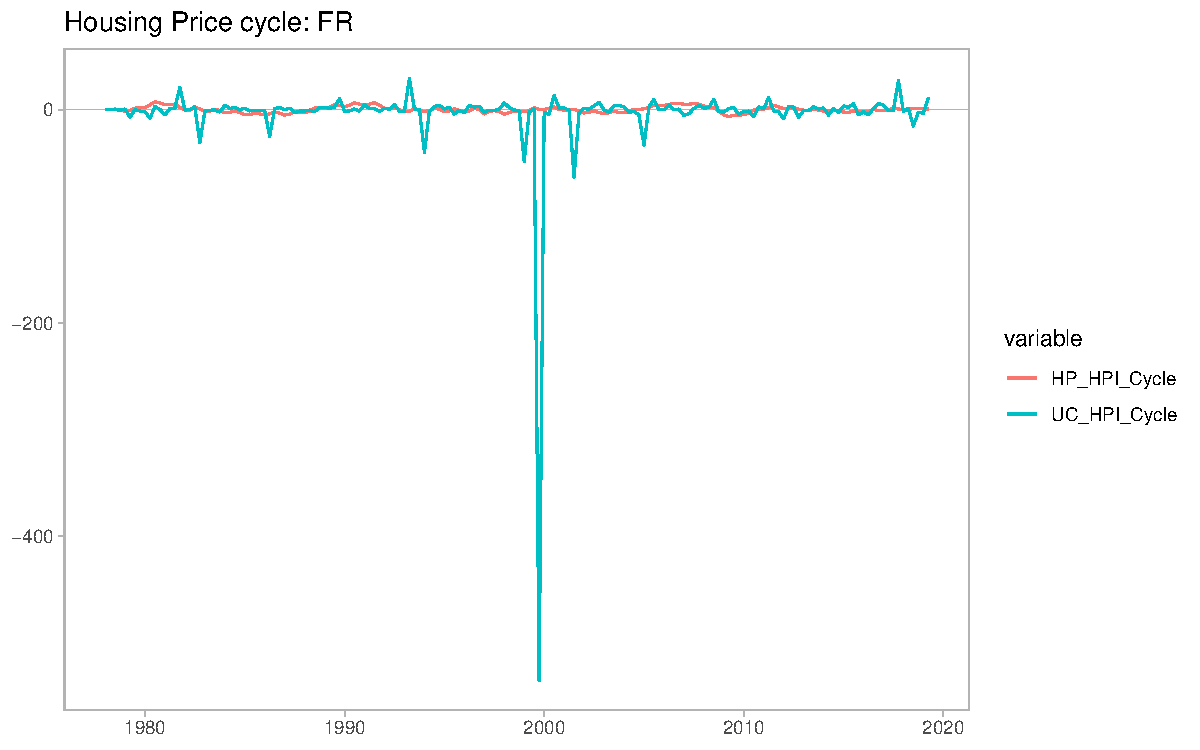
\includegraphics[scale=0.7]{../Output/Graphs/HP_cycle_FR.pdf}}
%	\centerline{\includegraphics[scale=0.7]{../Output/Graphs/HP_trend_FR.pdf}}
%\end{figure}
%
%
%\begin{figure}[h!]
%	\caption{Japan Credit components}	
%	\centerline{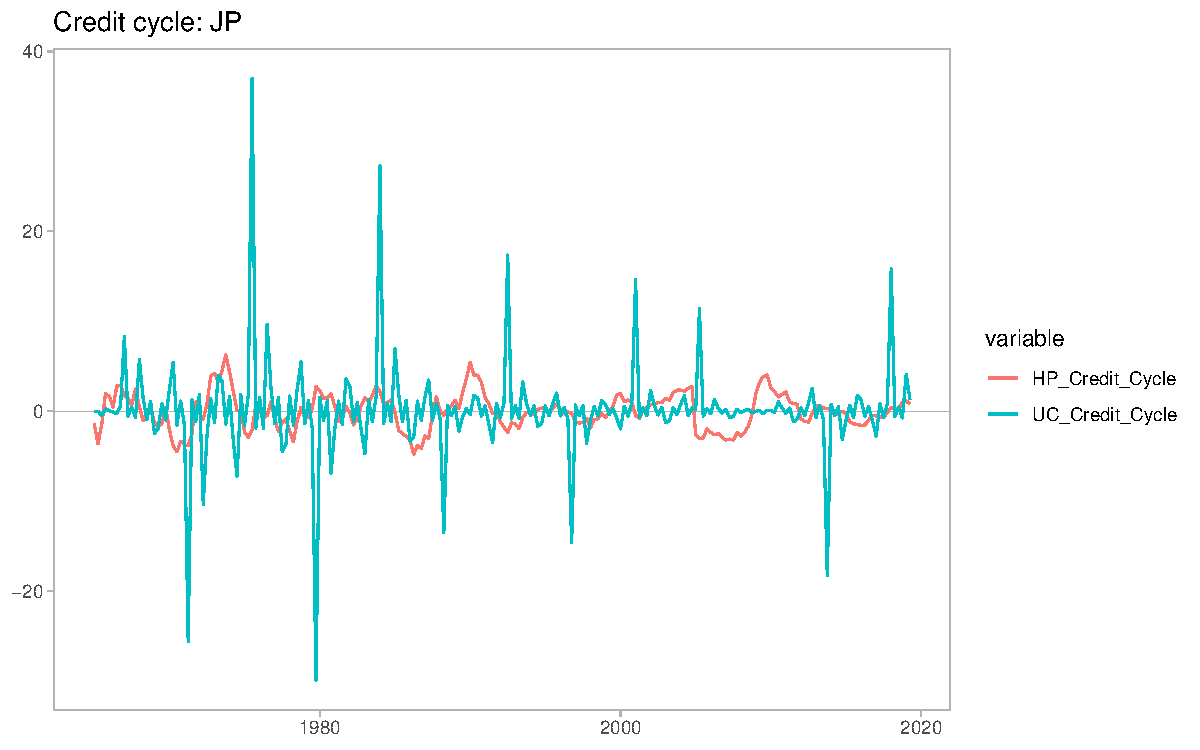
\includegraphics[scale=0.7]{../Output/Graphs/Credit_cycle_JP.pdf}}
%	\centerline{\includegraphics[scale=0.7]{../Output/Graphs/Credit_trend_JP.pdf}}
%\end{figure}
%
%\begin{figure}[h!]
%	\caption{Japan Housing Price components}	
%	\centerline{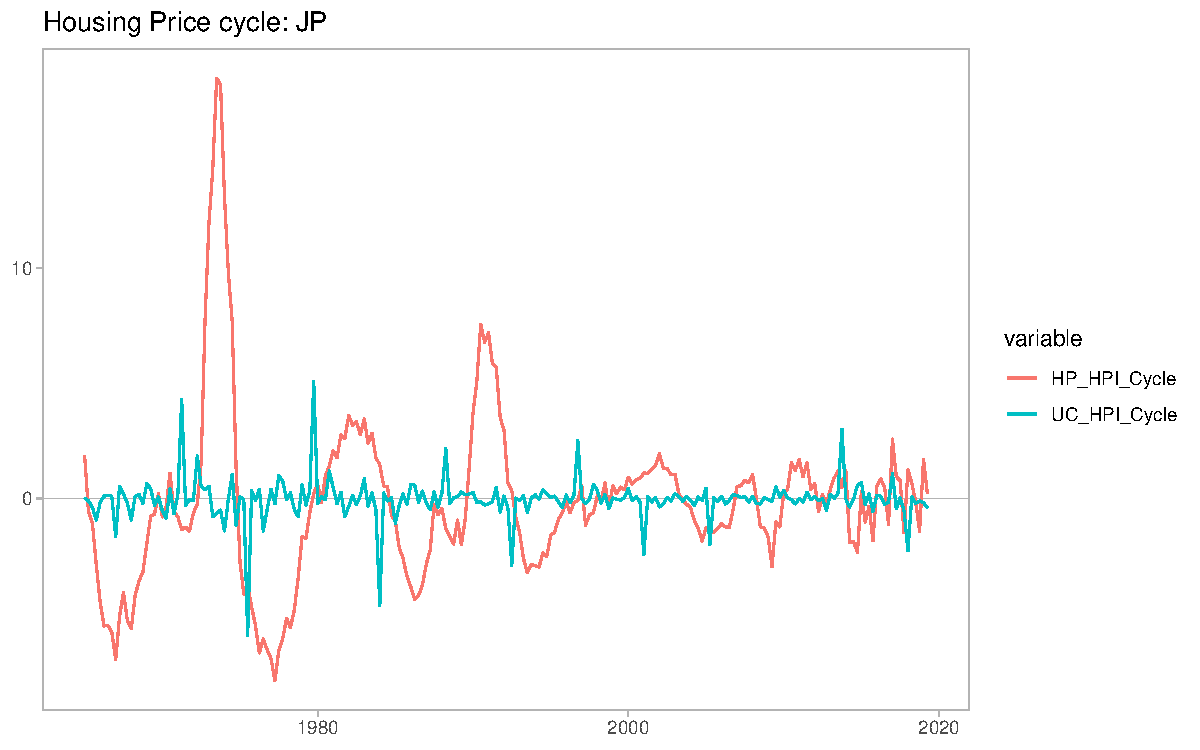
\includegraphics[scale=0.7]{../Output/Graphs/HP_cycle_JP.pdf}}
%	\centerline{\includegraphics[scale=0.7]{../Output/Graphs/HP_trend_JP.pdf}}
%\end{figure}
%
%
%\begin{figure}[h!]
%	\caption{Korea Credit components}	
%	\centerline{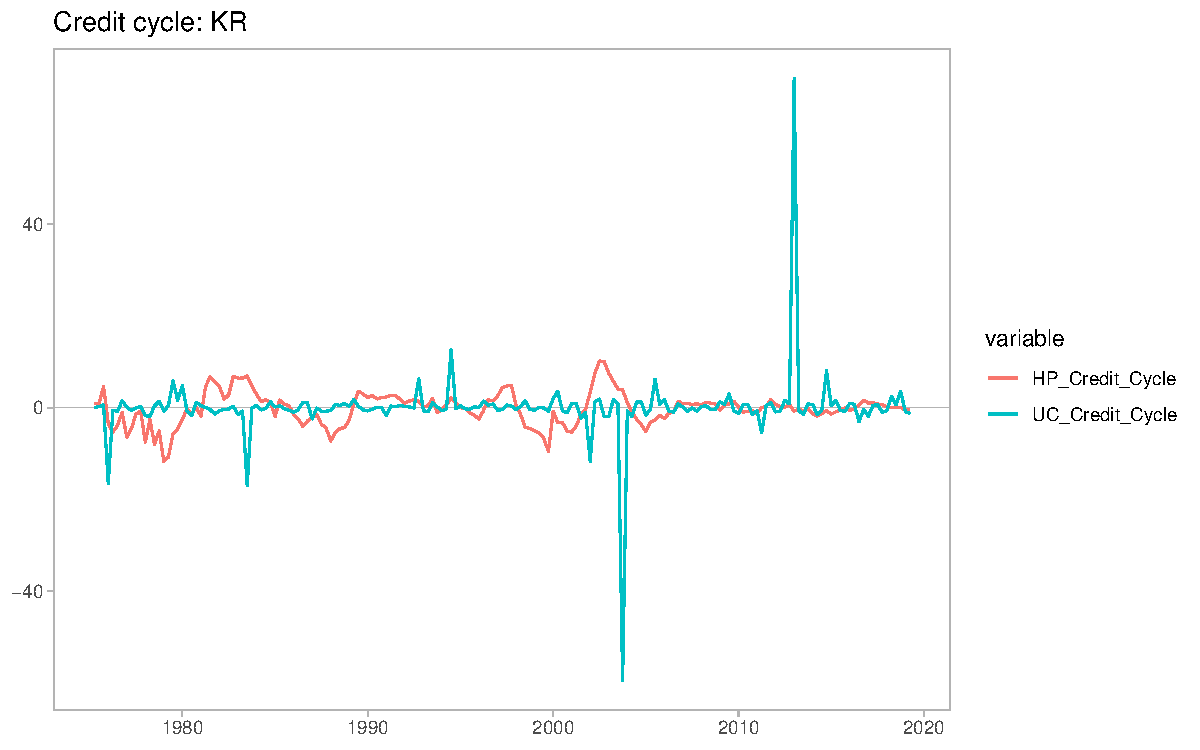
\includegraphics[scale=0.7]{../Output/Graphs/Credit_cycle_KR.pdf}}
%	\centerline{\includegraphics[scale=0.7]{../Output/Graphs/Credit_trend_KR.pdf}}
%\end{figure}
%
%\begin{figure}[h!]
%	\caption{Korea Housing Price components}	
%	\centerline{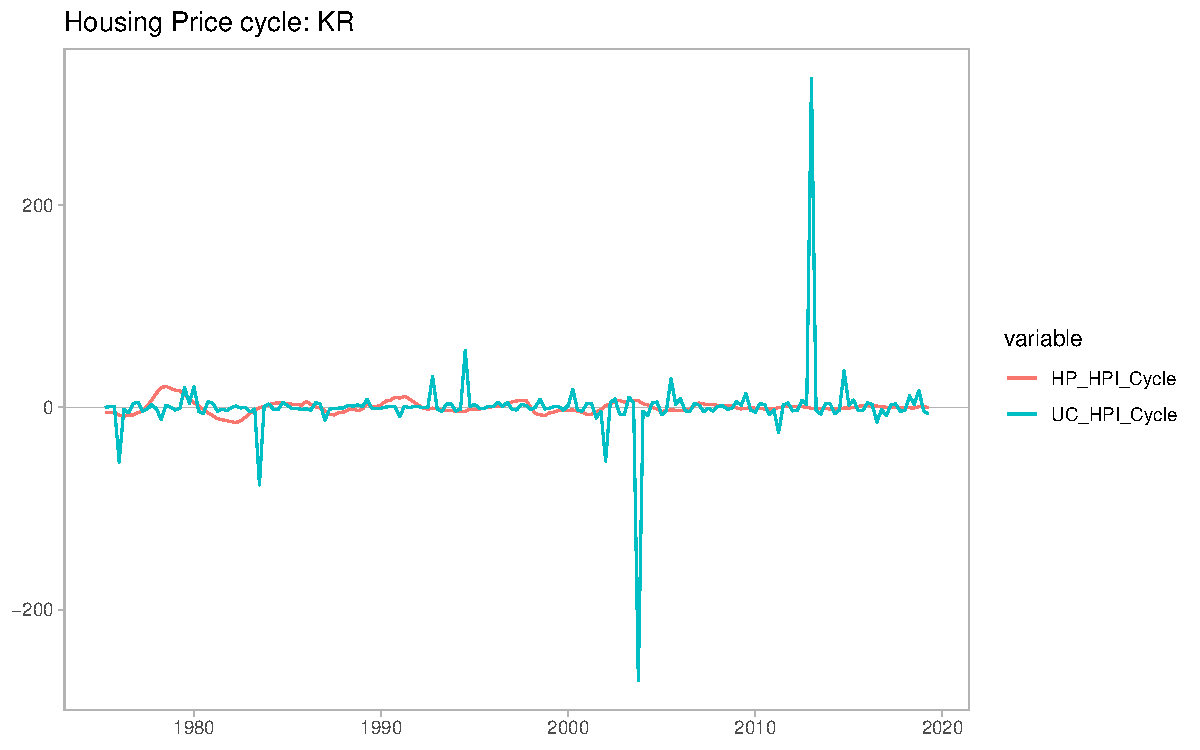
\includegraphics[scale=0.7]{../Output/Graphs/HP_cycle_KR.pdf}}
%	\centerline{\includegraphics[scale=0.7]{../Output/Graphs/HP_trend_KR.pdf}}
%\end{figure}

\clearpage
%
%\section{Impulse Response Function}
%
%
%
%This section show IRFs that are really unstable. I am guessing that is because the way I specify the function:
%
%Instead of normally having: $\psi_t = \phi^y_{11}*\psi_l + \phi^y_{12}*\psi_{ll}$
%
%I specify the IRF as: $\psi_t = \phi^y_{11}*\psi_l + \phi^y_{12}*\psi_{ll} + \phi^y_{21}*\psi_l + \phi^y_{22}*\psi_{ll} $
%\\
%This potentially causes the unstability in the following IRF graphs. Also the fact that the constraints for autoregressive parameters have not been optimally setup could cause the issue.
%
%
%\begin{figure}[h!]
%	\caption{US IRF}	
%	\centerline{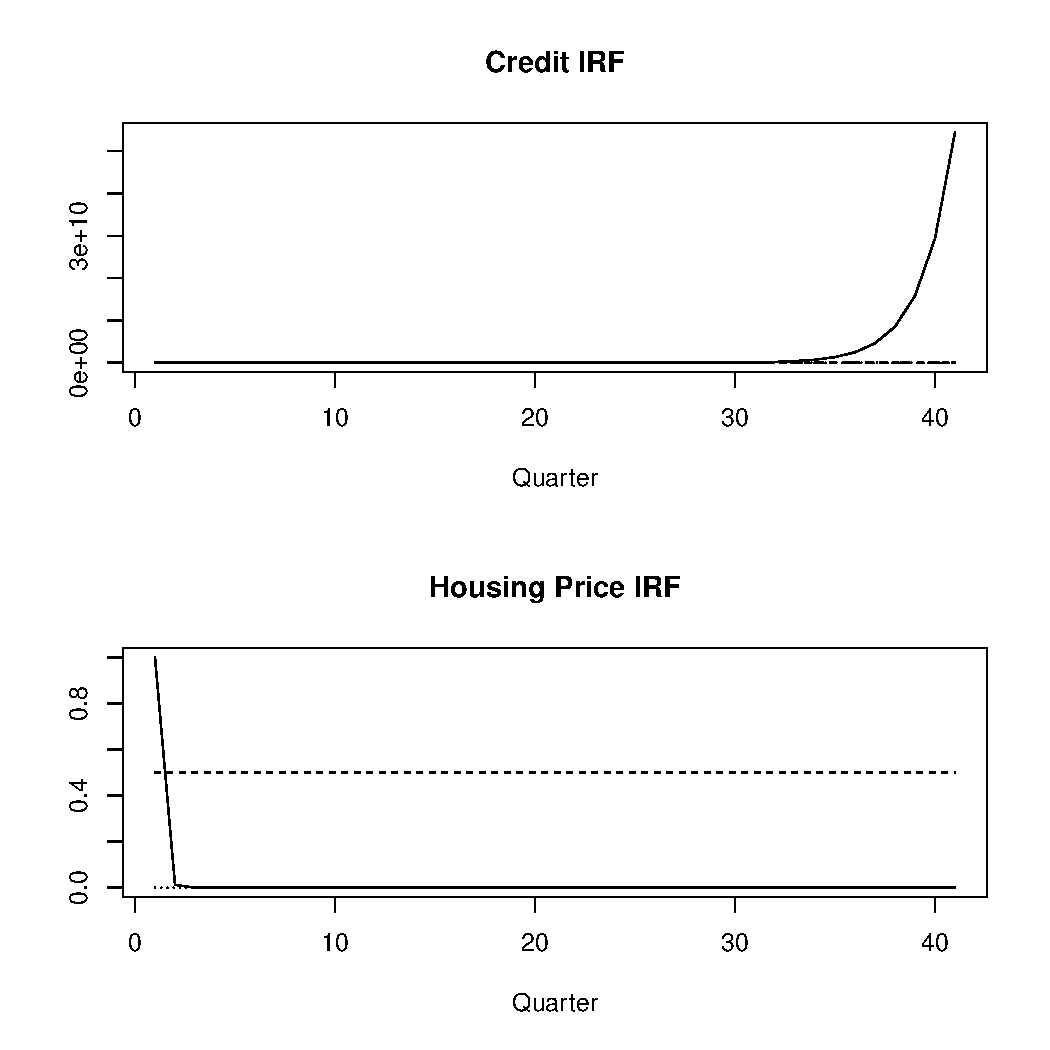
\includegraphics[scale=0.7]{../Output/Graphs/IRF_US.pdf}}
%\end{figure}
%
%\begin{figure}[h!]
%	\caption{UK IRF}	
%	\centerline{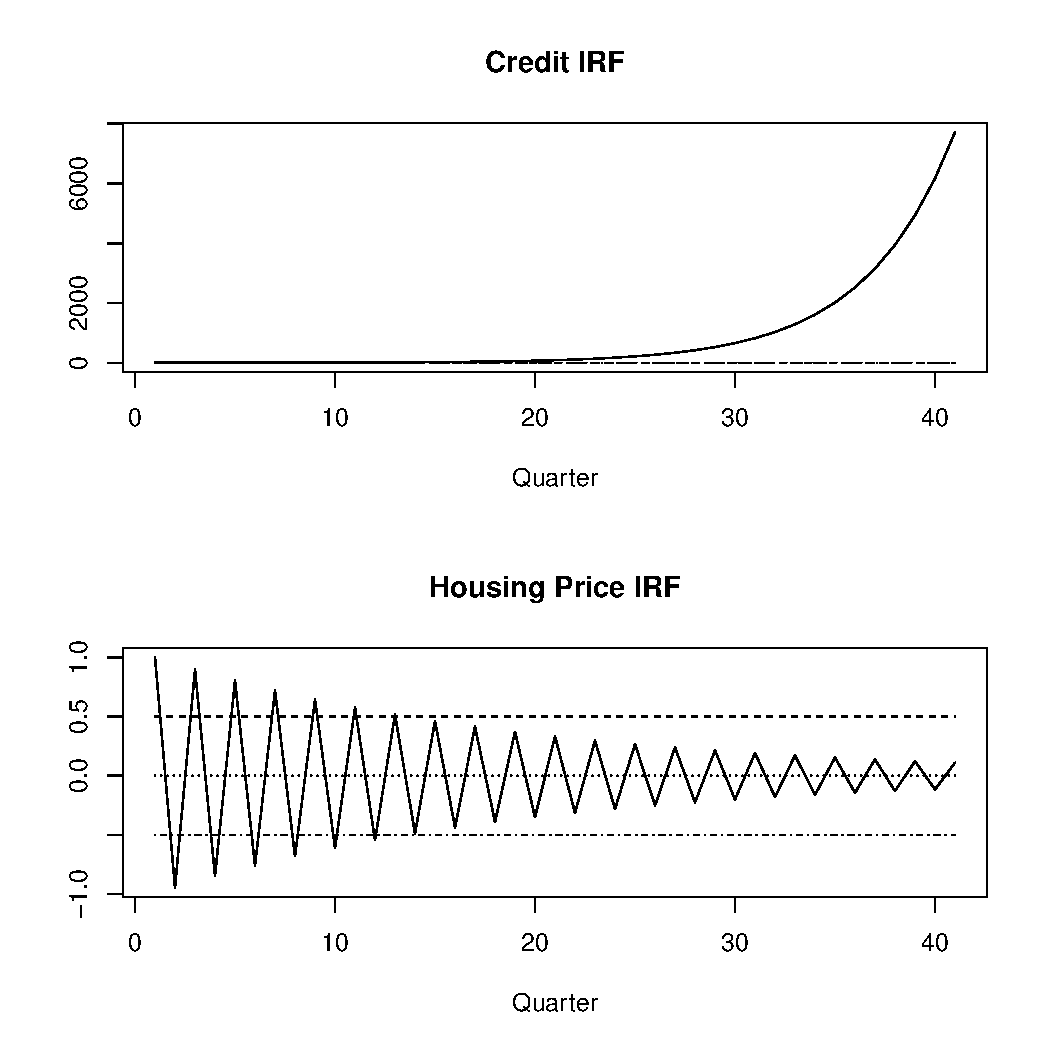
\includegraphics[scale=0.7]{../Output/Graphs/IRF_GB.pdf}}
%\end{figure}
%
%\begin{figure}[h!]
%	\caption{Germany IRF}	
%	\centerline{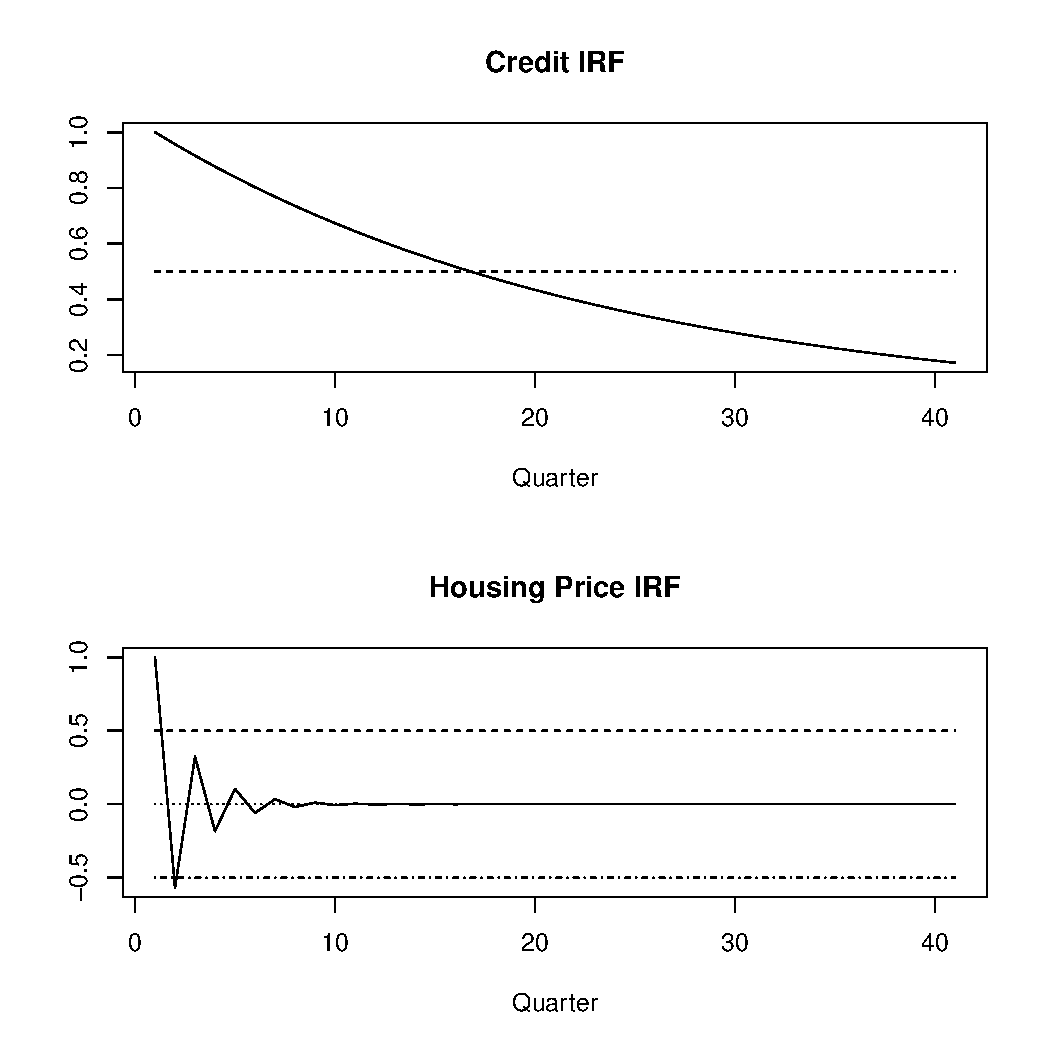
\includegraphics[scale=0.7]{../Output/Graphs/IRF_DE.pdf}}
%\end{figure}
%
%\begin{figure}[h!]
%	\caption{France IRF}	
%	\centerline{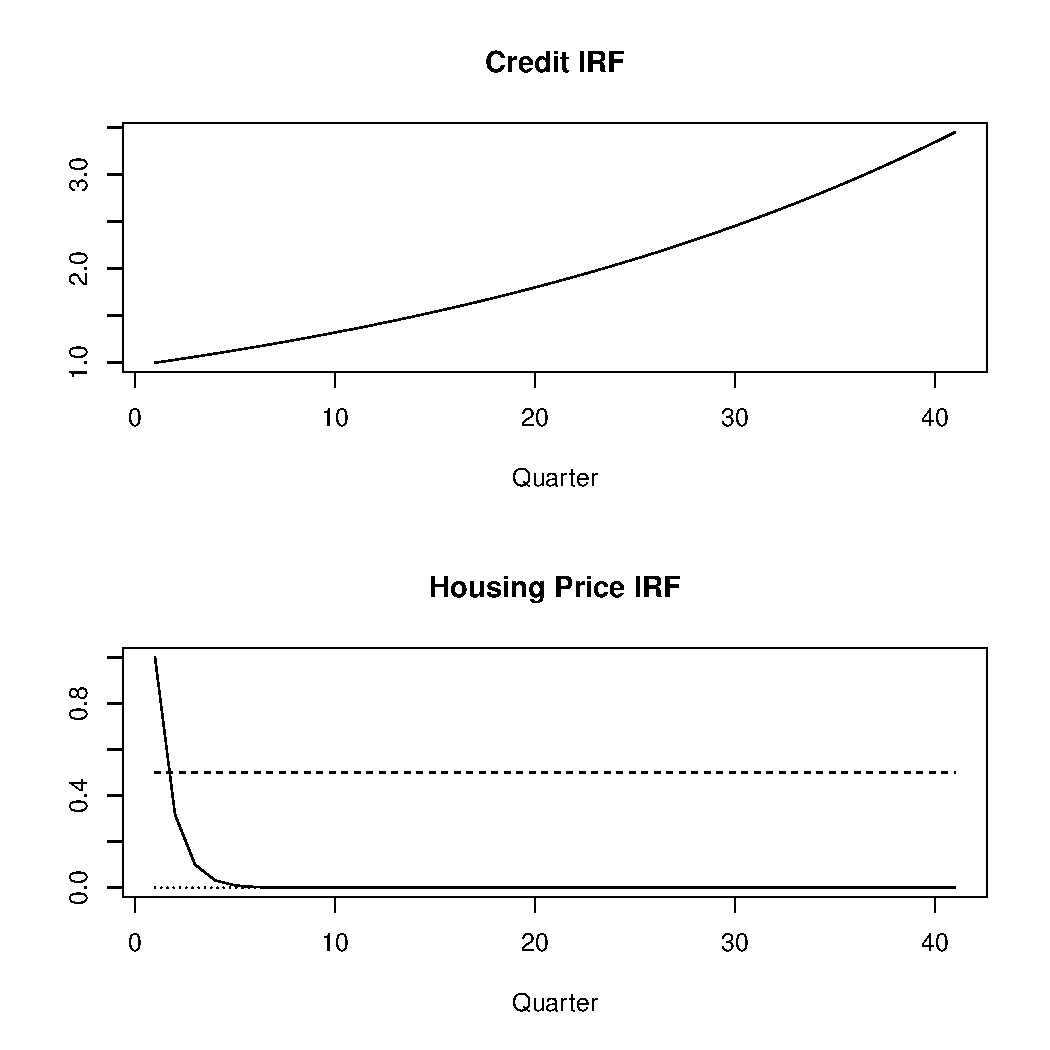
\includegraphics[scale=0.7]{../Output/Graphs/IRF_FR.pdf}}
%\end{figure}
%
%\begin{figure}[h!]
%	\caption{Japan IRF}	
%	\centerline{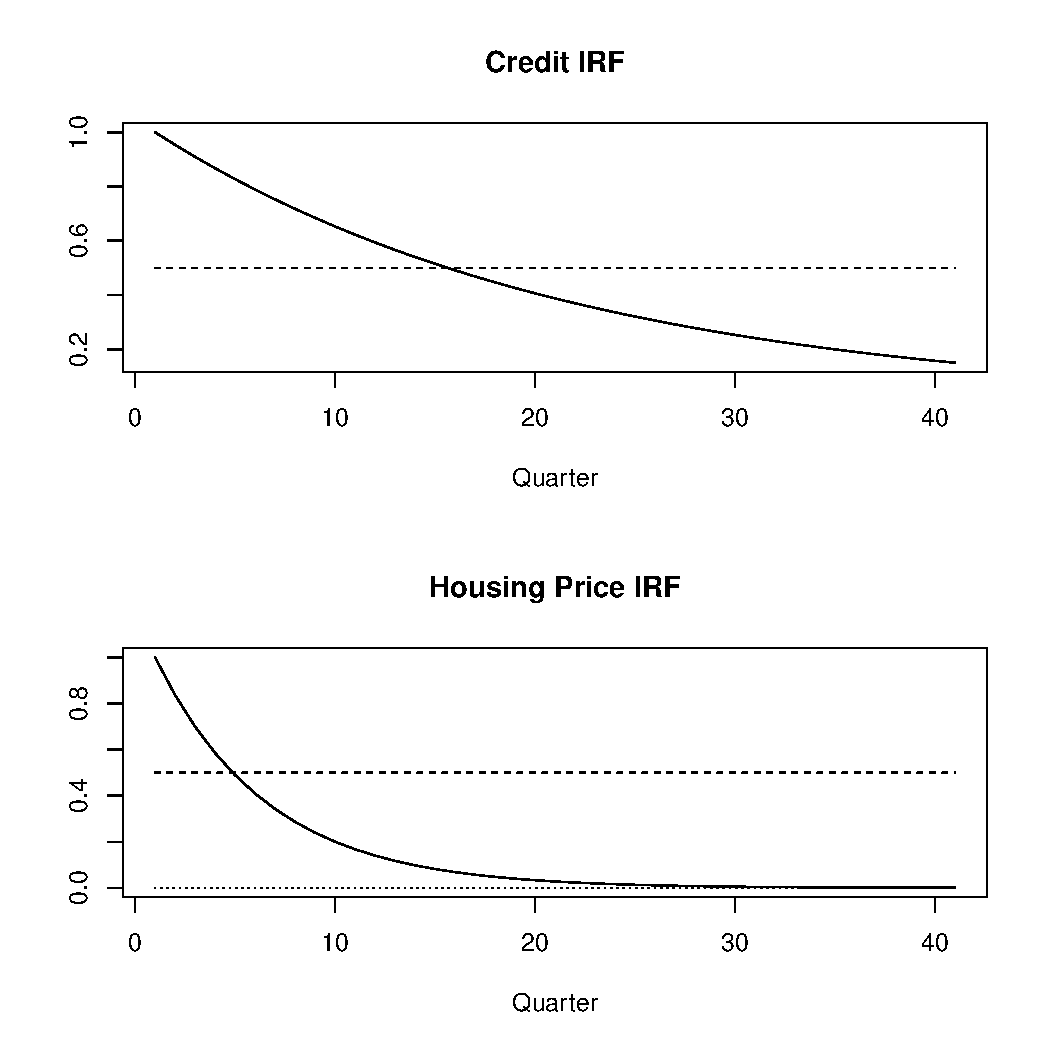
\includegraphics[scale=0.7]{../Output/Graphs/IRF_JP.pdf}}
%\end{figure}
%
%\begin{figure}[h!]
%	\caption{Korea IRF}	
%	\centerline{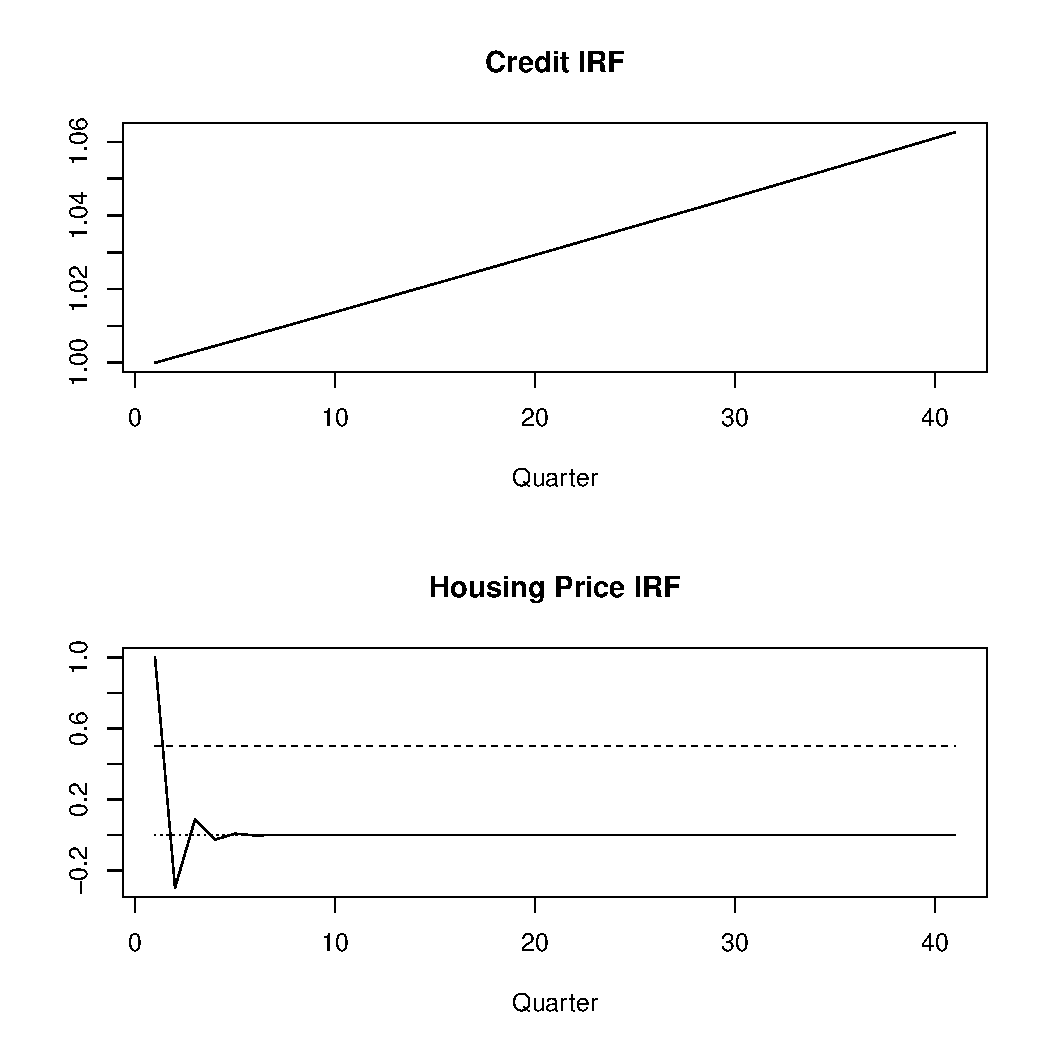
\includegraphics[scale=0.7]{../Output/Graphs/IRF_KR.pdf}}
%\end{figure}

\end{outline}
\end{document}